%%%%%%%%%%%%%%%%%%%%%%% file template.tex %%%%%%%%%%%%%%%%%%%%%%%%%
%
% This is a general template file for the LaTeX package SVJour3
% for Springer journals.          Springer Heidelberg 2010/09/16
%
% Copy it to a new file with a new name and use it as the basis
% for your article. Delete % signs as needed.
%
% This template includes a few options for different layouts and
% content for various journals. Please consult a previous issue of
% your journal as needed.
%
%%%%%%%%%%%%%%%%%%%%%%%%%%%%%%%%%%%%%%%%%%%%%%%%%%%%%%%%%%%%%%%%%%%
%
% First comes an example EPS file -- just ignore it and
% proceed on the \documentclass line
% your LaTeX will extract the file if required
\begin{filecontents*}{example.eps}
%!PS-Adobe-3.0 EPSF-3.0
%%BoundingBox: 19 19 221 221
%%CreationDate: Mon Sep 29 1997
%%Creator: programmed by hand (JK)
%%EndComments
gsave
newpath
  20 20 moveto
  20 220 lineto
  220 220 lineto
  220 20 lineto
closepath
2 setlinewidth
gsave
  .4 setgray fill
grestore
stroke
grestore
\end{filecontents*}
%
\RequirePackage{fix-cm}
%
%\documentclass{svjour3}                     % onecolumn (standard format)
%\documentclass[smallcondensed]{svjour3}     % onecolumn (ditto)
%\documentclass[smallextended]{svjour3}       % onecolumn (second format)
\documentclass[twocolumn]{svjour3}          % twocolumn
%
\smartqed  % flush right qed marks, e.g. at end of proof
%
\usepackage{graphicx}
%
\usepackage{mathptmx}      % use Times fonts if available on your TeX system
%
% insert here the call for the packages your document requires
%\usepackage{latexsym}
% etc.
\usepackage{color}
\usepackage{bbm}
\usepackage{enumitem}
\usepackage{calc}
\usepackage{multirow}
\usepackage{xspace}
\usepackage{booktabs}
%
% please place your own definitions here and don't use \def but
% \newcommand{}{}
\newcommand{\figref}[1]{Fig\onedot~\ref{#1}}
\newcommand{\equref}[1]{Eq\onedot~\eqref{#1}}
\newcommand{\secref}[1]{Sec\onedot~\ref{#1}}
\newcommand{\tabref}[1]{Tab\onedot~\ref{#1}}
\newcommand{\thmref}[1]{Theorem~\ref{#1}}
\newcommand{\prgref}[1]{Program~\ref{#1}}
\newcommand{\algref}[1]{Alg\onedot~\ref{#1}}
\newcommand{\clmref}[1]{Claim~\ref{#1}}
\newcommand{\lemref}[1]{Lemma~\ref{#1}}
\newcommand{\ptyref}[1]{Property\onedot~\ref{#1}}
\newcommand{\ve}[1]{{\mathbf #1}} % for displaying a vector or matrix
\newcommand{\hua}[1]{{\mathcal #1}}
\newcommand{\by}[2]{\ensuremath{#1 \! \times \! #2}}
%
% Insert the name of "your journal" with
\journalname{International Journal of Computer Vision}
%
\begin{document}

\title{Pose-Guided and Scale-Aware Human Semantic Part Segmentation in Natural Multi-Person Scenes
%\thanks{Grants or other notes
%about the article that should go on the front page should be
%placed here. General acknowledgments should be placed at the end of the article.}
}

%\subtitle{Do you have a subtitle?\\ If so, write it here}

%\titlerunning{Short form of title}        % if too long for running head

\author{Fangting Xia         \and
        Peng Wang \and
        Alan Yuille %etc.
}

%\authorrunning{Short form of author list} % if too long for running head

\institute{Fangting Xia \at
              Google Inc. \\
              \email{sukixia@gmail.com}           %  \\
%             \emph{Present address:} of F. Author  %  if needed
           \and
           Peng Wang \at
              Baidu Inc. \\
              \email{pengwangpku2012@gmail.com}
           \and
           Alan Yuille \at
              Johns Hopkins University \\
              \email{alan.yuille@jhu.edu}
}

\date{Received: date / Accepted: date}
% The correct dates will be entered by the editor

\maketitle

\begin{abstract}
Parsing articulated objects like humans into semantic part regions (e.g. head, body and arms, etc.) from a natural image is a fundamental yet challenging problem in computer vision.
The major difficulties of this problem derive from multi-instance confusion and large variability in human pose and scale.
Current state-of-the-art methods use deep neural networks to predict part labels directly, and then refine the labels by a graphical model such as the dense CRF.
These methods are still limited in complex natural scenes because they have no efficient mechanisms to handle multi-person overlapping or to adapt to the scale of human instances.
In this work, we propose a part segmentation framework that handles these hurdles effectively.
Our framework is scale-aware: we design an hierarchical ``auto-zoom" strategy to allow the model to adapt to the size of human instances and their corresponding parts.
Our framework is also pose-guided: it predicts human pose and part segmentation jointly, letting the two tasks benefit each other.
We extend the PASCAL VOC part datasets with pose joints and perform extensive experiments on it.
We show that our method achieves state-of-the-art part segmentation performance, and is especially better at handling small human instances and small parts.       

\keywords{semantic part segmentation \and pose estimation \and auto-zoom}
%\PACS{PACS code1 \and PACS code2 \and more}
%\subclass{MSC code1 \and MSC code2 \and more}
\end{abstract}

\section{Introduction}
\label{intro}
% What humans do to perform semantic part segmentation. Pose estimation is a correlated task.
When people look at natural images, they often first locate regions that contain objects, and then zoom in or out on the object regions to perform the more detailed task of object semantic part segmentation, i.e. decomposing each object instance region into its semantic parts (e.g. head, body, lower-arms, etc.).
A closely correlated task to object semantic part segmentation is object pose estimation, which aims to predict the position of joints (e.g. forehead, neck, left shoulder, etc.) for each object instance.
Though closely correlated, semantic part segmentation~\cite{rauschert2012generative,long2015fully,wang2015joint,chen2016deeplab} and pose estimation~\cite{yang2011articulated,tompson2015efficient,chen2015parsing} are studied individually most of the time. They are both crucial to object interaction understanding and many high-level tasks, e.g. fine-grained recognition~\cite{branson2014bird,zhang2014part,krause2016unreasonable}, action recognition~\cite{wang2012discriminative,zhou2015interaction,chunyu_action}, person identification~\cite{ma2011human,zhao2017deeply}, and video surveillance~\cite{gallego2008segmentation,liu2017surveillance}. 

\begin{figure}
 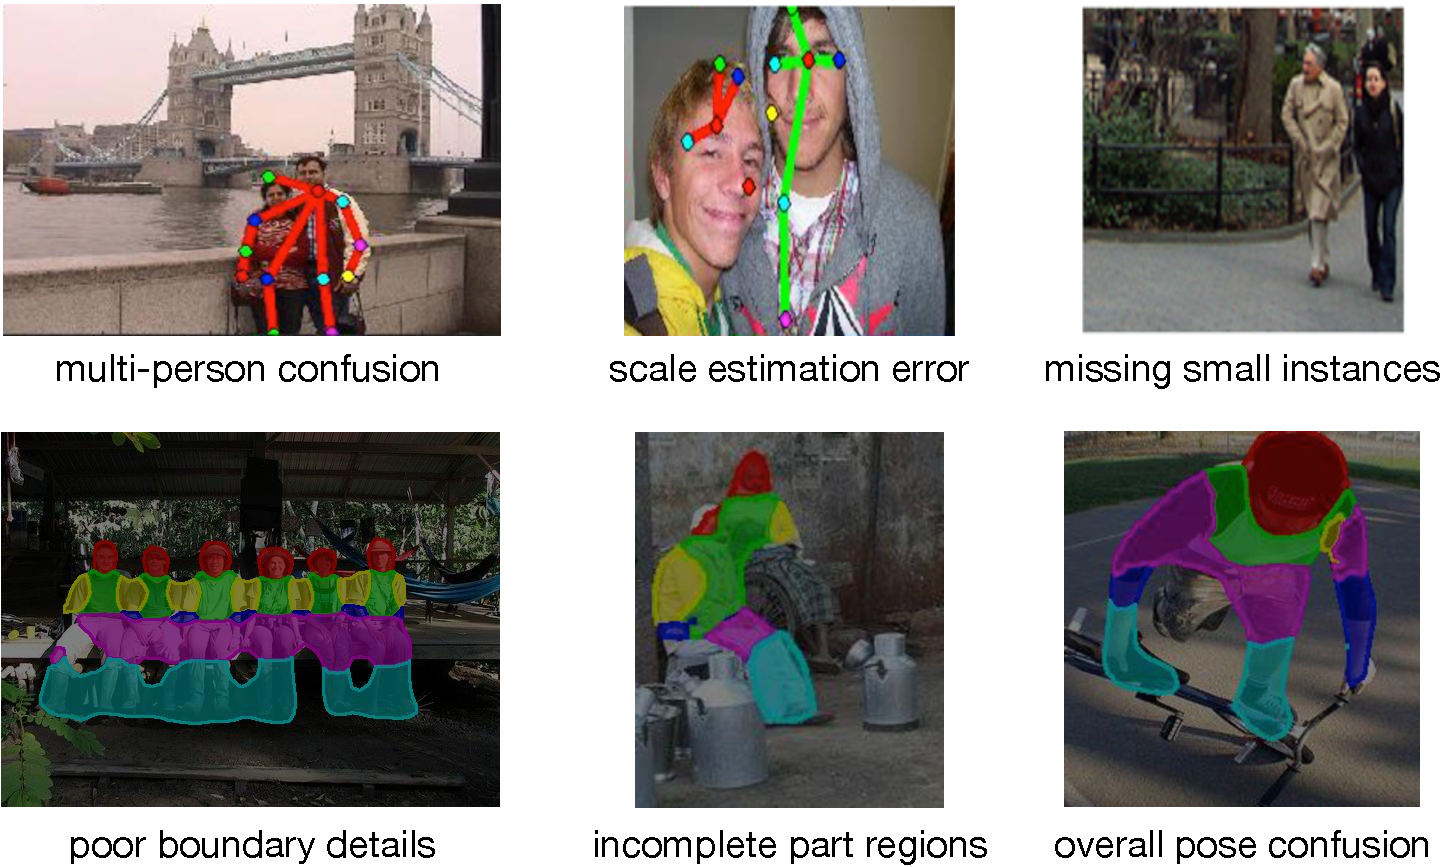
\includegraphics[width=1.0\linewidth]{figs/intro_hard.pdf}
\caption{Challenges for current human pose estimation algorithms (top row) and semantic part segmentation algorithms (bottom row) in natural multi-person scenes.}
\label{fig:challenge}
\end{figure}

\begin{figure*}
\begin{center}
 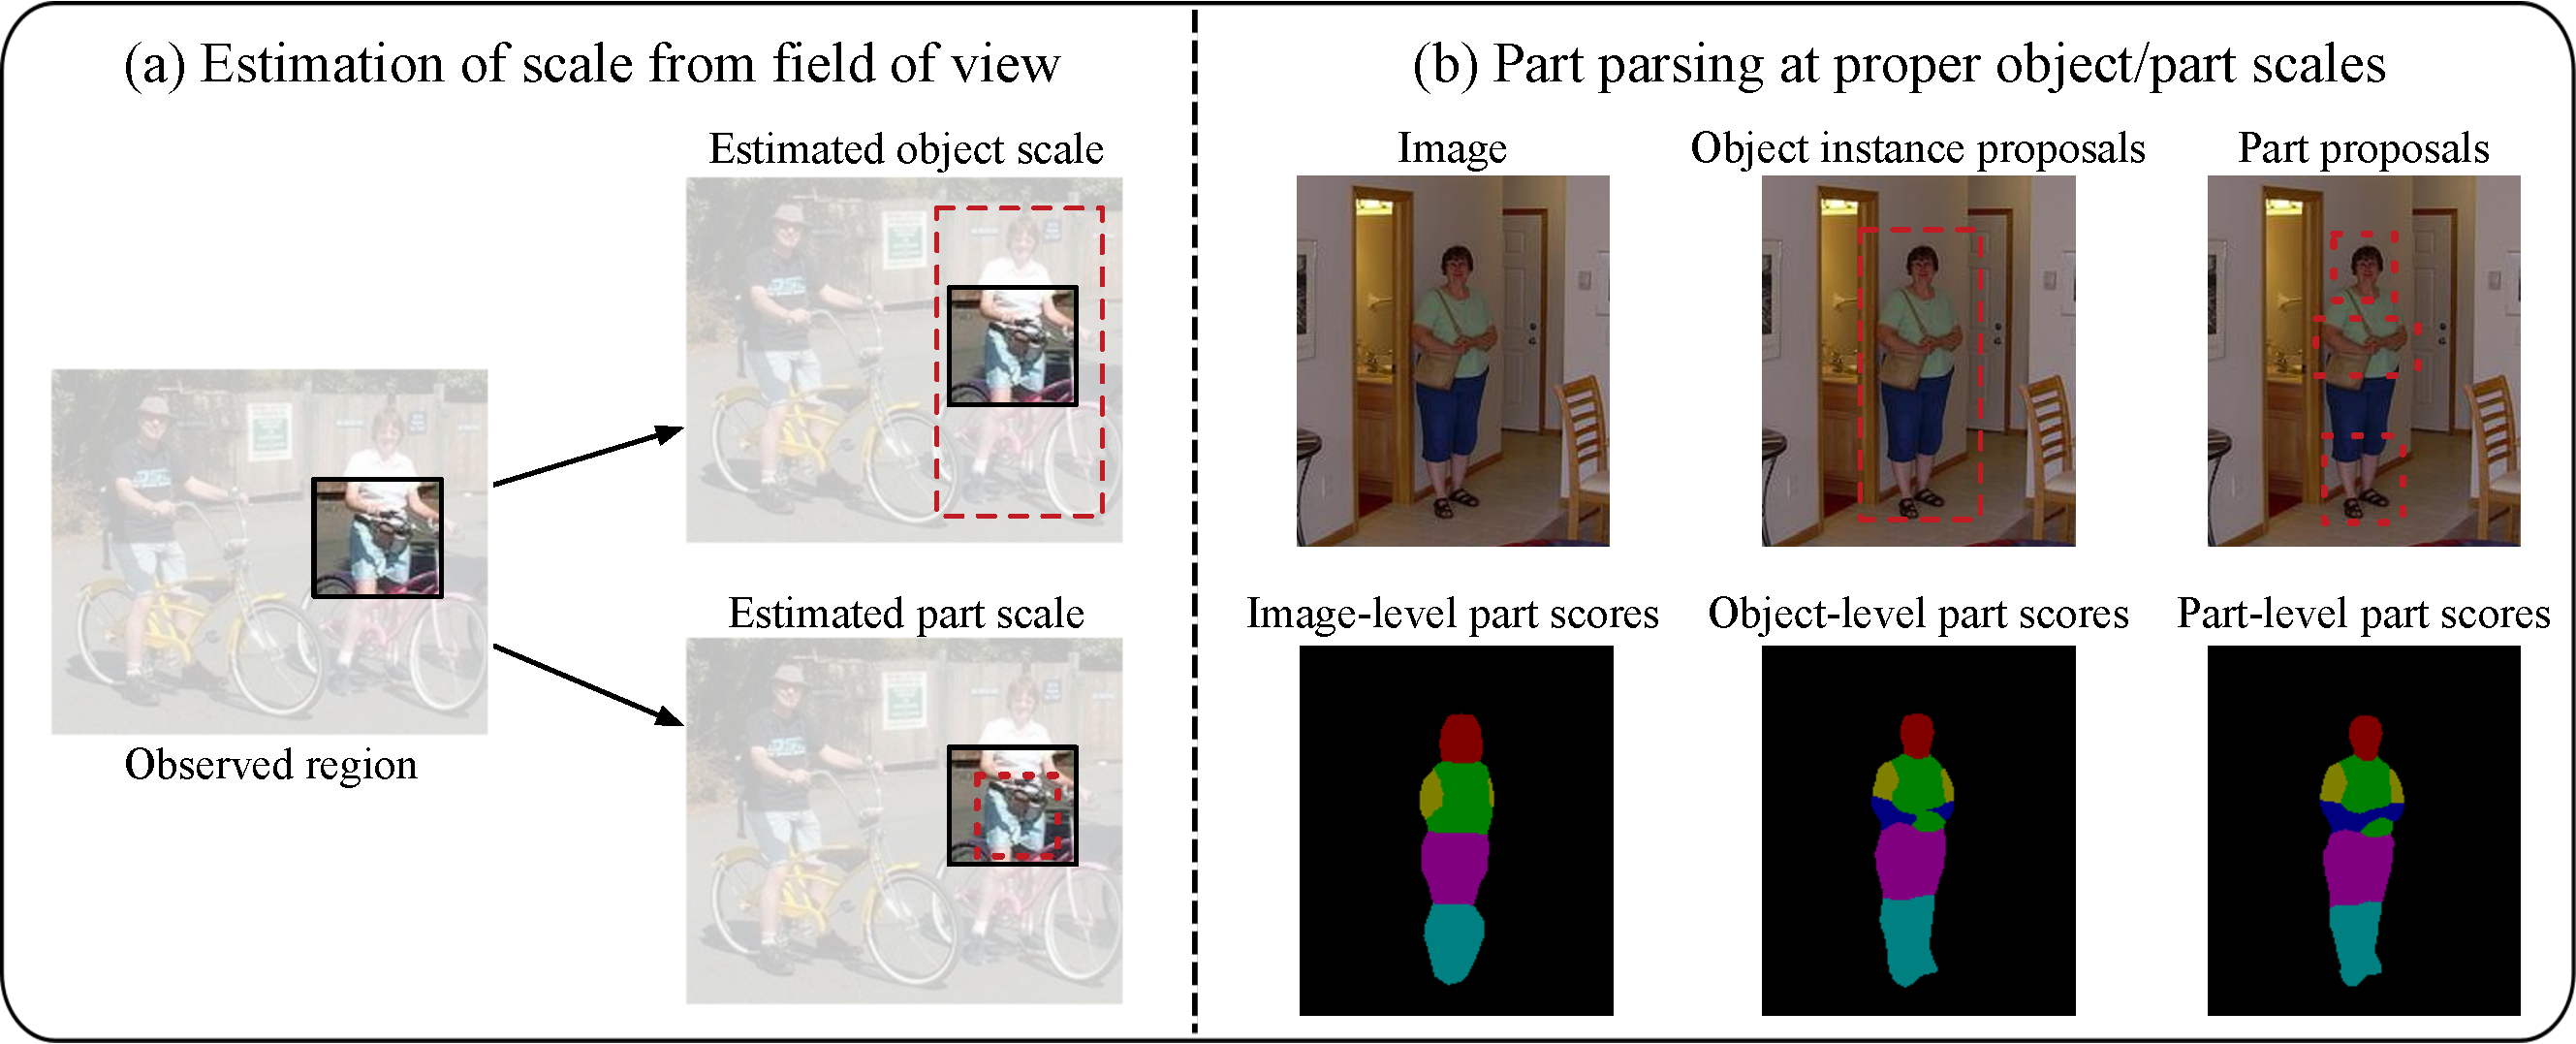
\includegraphics[width=0.8\textwidth]{figs/intuition_eccv.pdf}
\end{center}
\caption{Intuition of our hierarchical auto-zoom model (HAZN), which handles the large variation of object and part scale in natural multi-person scenes. (a) The scale
and location of an object and its parts (the red dashed boxes) can be estimated
from the observed field of view (the black solid box) of a neural network. (b)
Part segmentation can be more accurate by using proper object and part scales. In the top row, we show our estimated object and part scales. In the bottom row,
our part segmentation results gradually become better by increasingly utilizing the
estimated object and part scales.}
\label{fig:motivation_eccv}
\end{figure*}

% Difficulty of both tasks. Current methods and their shortcomings.
Currently, both semantic part segmentation and pose estimation face unsolved challenges in natural multi-person scenes (see Fig.~\ref{fig:challenge}).
Traditional semantic part segmentation methods~\cite{bo2011shape,eslami2012generative,yamaguchi2012parsing,dong2013deformable,zhu2011max} usually generate part segment proposals first and then use graphical models to select and assemble the part segment proposals into human instances. These methods are often time-consuming and only work well in constrained scenes, which pre-suppose known scale, fairly accurate localization, clear appearances, and/or relatively simple poses. Recently, dramatic progress has been made in semantic part segmentation due to the advent of fully convolutional neural networks (FCNs)~\cite{long2015fully} and the availability of object part annotations in large-scale datasets like PASCAL~\cite{chen2014detect}. These FCN-based methods~\cite{hariharan2015hypercolumns,wang2015joint,chen2016deeplab} usually compute pixel-wise part labels directly in a simple and fast way, and then optionally refine the labels by a graphical model such as the dense CRF~\cite{krahenbuhl2011efficient}. Although these FCN-based methods work well generally, they still suffer from the following two problems when handling natural multi-person scenes. They can make mistakes (e.g. missing small instances, producing poor boundary details or incomplete part regions, etc.) on small scale or extra large scale human instances for short of an effective mechanism to adapt to the size of the object instance. They also tend to produce erroneous predictions when the human instance is in an unusual pose or the appearance cues are weak, due to lack of object-level shape prior to regularize the part segments.

Similar to the trend of semantic part segmentation, traditional pose estimation approaches adopt graphical models to combine spatial constraints with local observations of joints, based on low-level features, like color intensities, HOG~\cite{dalal2005histograms}, shape-context~\cite{belongie2001shape}, and so on. Recent strategies rely on deep-learned joint detectors, and use a carefully designed graphical model to select and assemble joints into valid pose
configurations. Traditional approaches suffer from limited feature representation power and can only work in simple datasets with small pose and scale variation. Recent deep-based approaches have much better invariance to pose/scale variation, but their localization of joints is still inaccurate (e.g. joints are sometimes outside the human body) and they still struggle in multi-person overlapping scenes.

% Two main models in our framework.
In this paper, we present a scale-aware and pose-guided part segmentation framework that effectively improves human semantic part segmentation in natural images with large pose/scale variation. The framework mainly contains two novel models: (1) a hierarchical auto-zoom model (HAZN) that handles the large scale variation of human instances and human parts; (2) a joint prediction model that combines pose estimation and semantic part segmentation together, letting the two tasks benefit each other. Here we give a brief introduction to the two proposed models.

% Intuition of HAZN
The hierarchical "auto-zoom" model (HAZN) model is a FCN-based model performing object/part scale estimation and part segmentation at the same time, adapting to the size of objects and parts. It's partially motivated by the proposal-free end-to-end detection strategies~\cite{huang2015densebox,liang2015proposal,ren2015faster,redmon2016you}. To get some intuition of this approach, observe in Fig.~\ref{fig:motivation_eccv}(a), that the scale and location of a target object, and of its corresponding
parts, can be estimated accurately from the field-of-view (FOV) window
by applying a deep neural network. Using estimated object and part scales, the semantic part segmentation results can become better and better, see Fig.~\ref{fig:motivation_eccv}(b). Please refer to Sec.~\ref{sec:hazn} for a detailed explanation of the HAZN model. 

\begin{figure}
 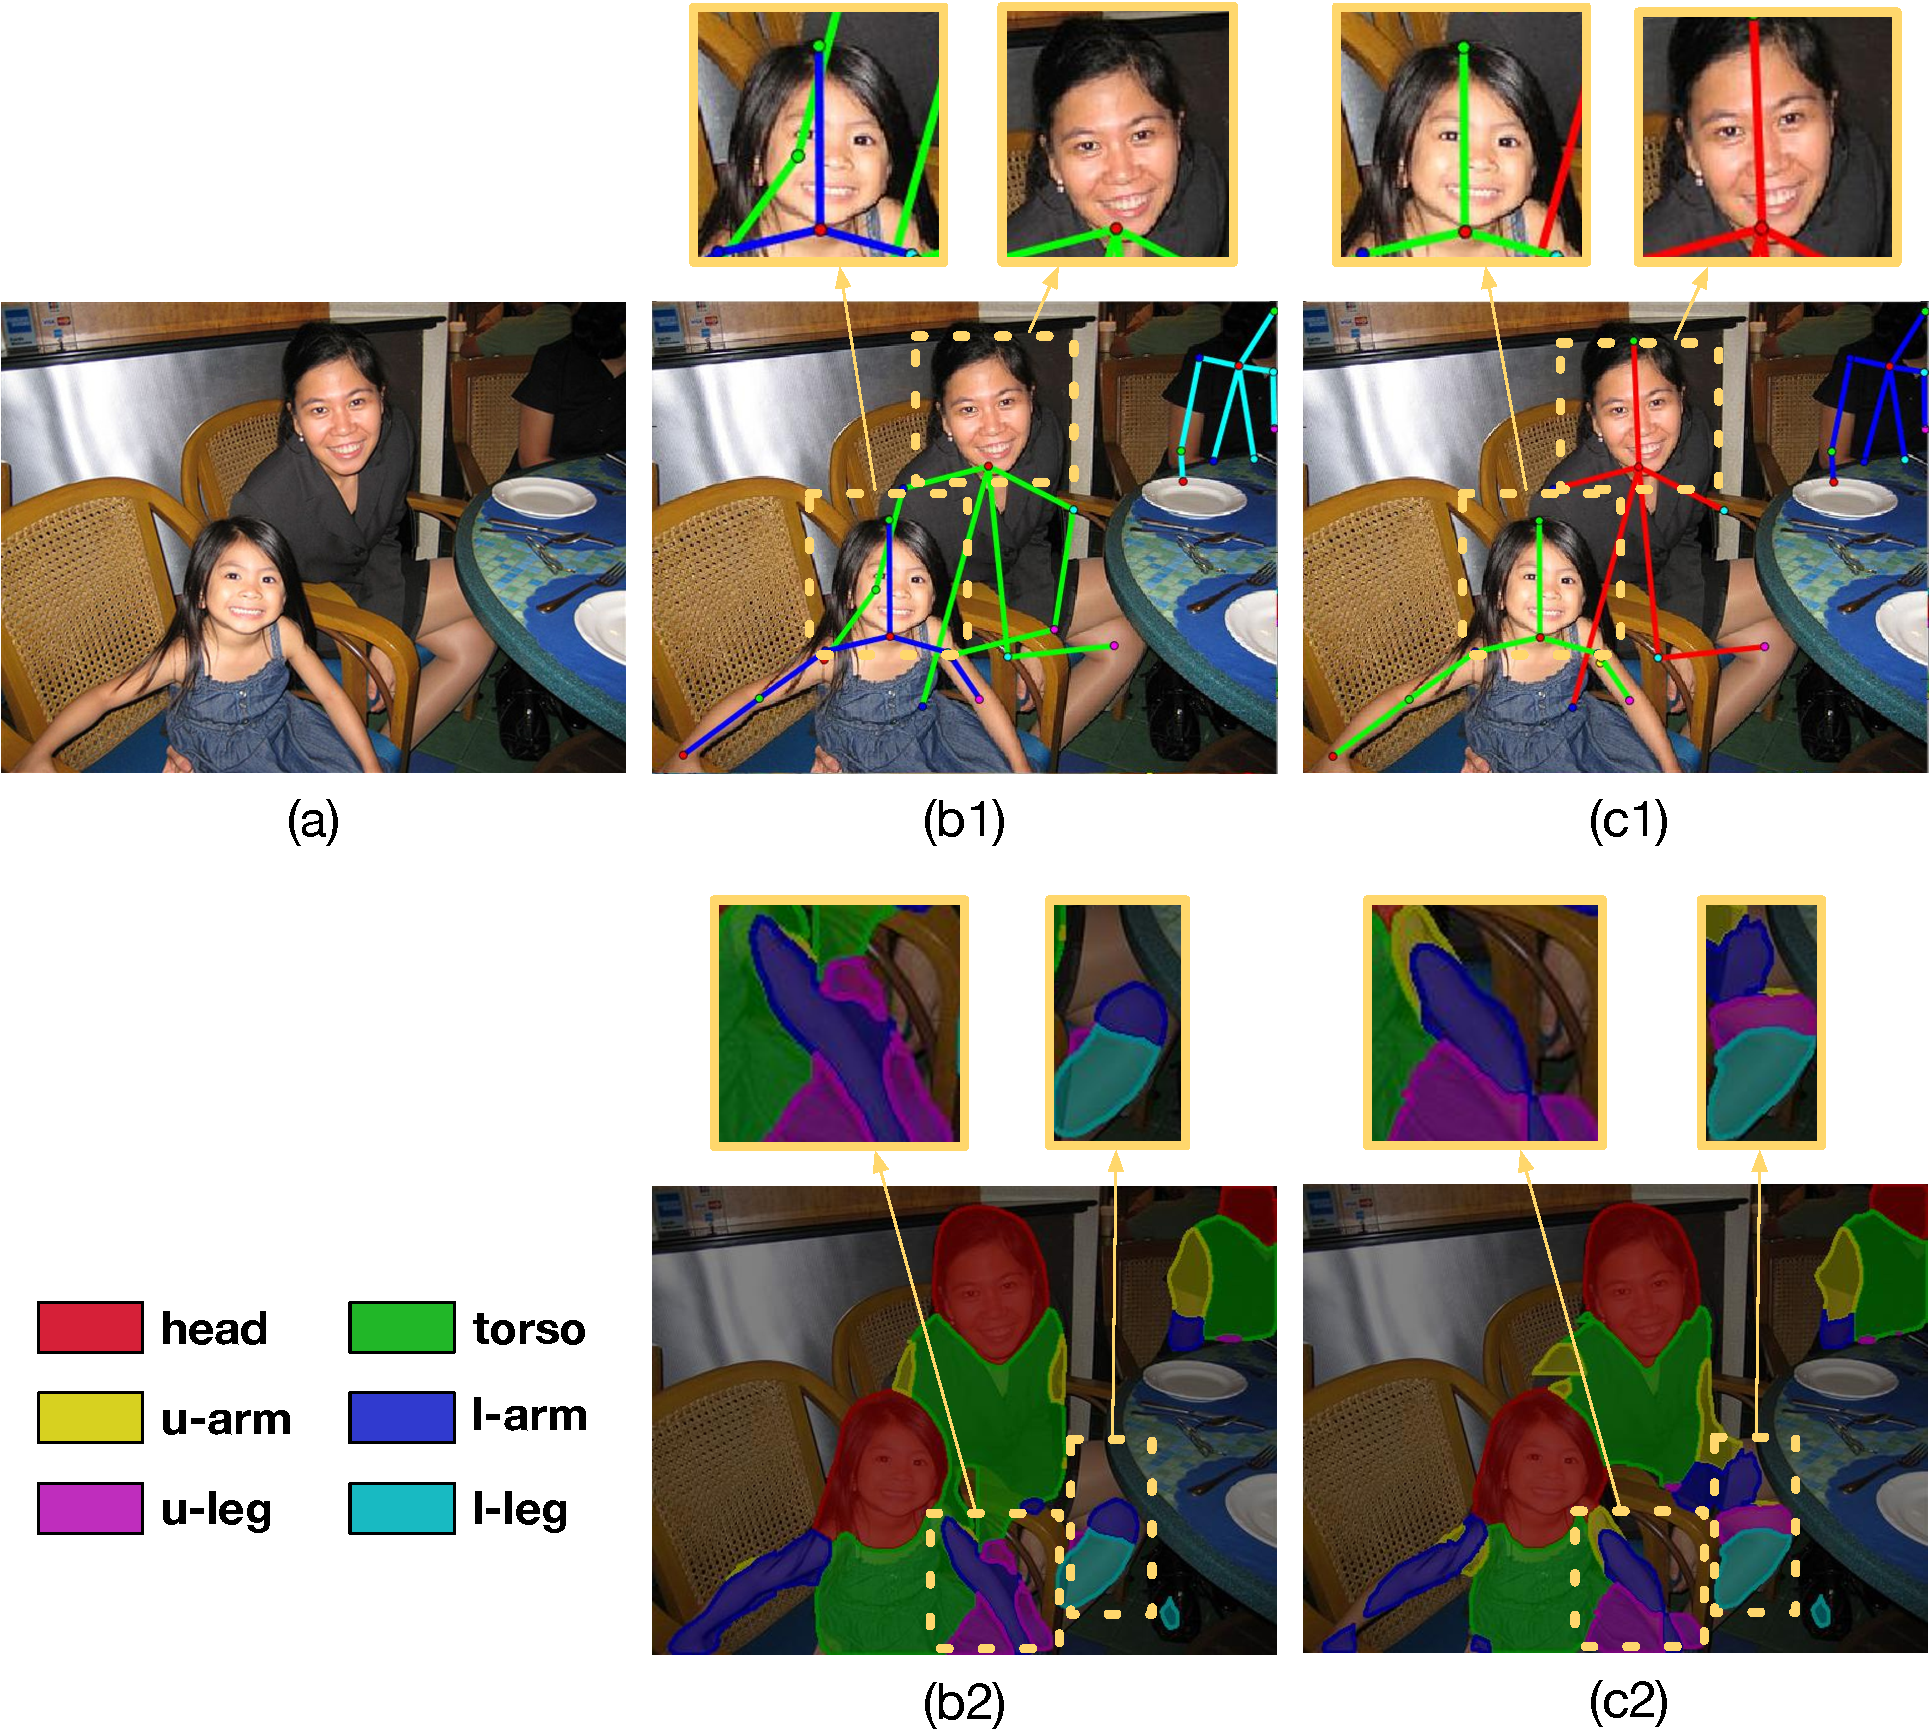
\includegraphics[width=1.0\linewidth]{figs/intuition_cvpr.pdf}
\caption{Joint human pose estimation and semantic part segmentation improve both tasks. (a) input image. (b) pose estimation and semantic part segmentation results before joint inference. (c) pose estimation and semantic part segmentation results after joint inference. Note that comparing (b1) and (c1), our result recovers the missing forehead joint and corrects the location error of right elbow and right wrist for the woman on the right. Comparing (b2) and (c2), our result gives more accurate details of lower arms and upper legs than (b2) for both people.}
\label{fig:motivation_cvpr}
\end{figure}

% Intuition of joint prediction model.
The joint prediction model is also a FCN-based framework aiming to solve the pose estimation task and the semantic part segmentation task jointly, in which the estimated pose provides object-level shape prior to regularize part segments (e.g. helping part segments align with human instances over the details of arms and legs where appearance cues are missing) while the part-level segments constrain the variation of pose locations (e.g. helping pose joints locate within their corresponding part segments). As shown in Fig.~\ref{fig:motivation_cvpr}, by taking advantage of the complementary property between pose estimation and semantic part segmentation, this joint prediction model produces better results on both tasks. See Sec.~\ref{sec:pose_and_seg} for detailed introduction of the model.

% Evaluation dataset and experiments.
In this paper, we address the task of human semantic part segmentation in ``the wild" where there are large variations in scale, pose, location, and occlusion. This motivates us to work with PASCAL images~\cite{everingham2014pascal} because these were chosen for studying multiple visual tasks, do not suffer from dataset design bias~\cite{li2014secrets}, and include large variations of objects, particularly of scale and pose. Hence human semantic part segmentation in PASCAL is considerably more difficult than in datasets, such as Fashionista~\cite{yamaguchi2012parsing}, that were constructed solely to evaluate human parsing. 

We illustrate our approach by extensive experiments on PASCAL-Person-Part dataset~\cite{chen2014detect}, which contains detailed part annotations for every person in a subset of PASCAL VOC 2010. We further augment this dataset with 14 pose joint locations through manual labeling to evaluate our joint prediction model. Our experiments show that our approach outperforms previous state-of-the-art methods for both semantic part segmentation and pose estimation tasks. We are particularly good at recovering small human parts, giving clearer details of arms and legs, and correcting local confusions of people.

\section{Related Works}
As human semantic part segmentation and human pose estimation are two fundamental topics in computer vision, many graphical models on the two topics have been proposed during the past thirty years. With the advent of powerful deep learning techniques, some models start to use deep-learned features, or even perform the whole task within a deep neural network. Recently, there are also works that combine pose estimation and segmentation in graphical models. In this section, we give an overall review of previous literature in these aspects.

\subsection{Human Semantic Part Segmentation}
Traditional methods on human semantic part segmentation fall into two major categories.
One type of methods first generate region/segment proposals for each semantic part, then select and assemble the region proposals by a graphical model.
Bo et al.~\cite{bo2011shape} generate region proposals by UCM segmentation~\cite{arbelaez2009contours}, rank the region proposals using shape and appearance features, and assemble the proposals with simple geometric constraints.
Dong et al.~\cite{dong2013deformable} get region proposals by UCM and CPMC~\cite{carreira2012cpmc}, extract a rich set of appearance features for each region proposal encoded by Fisher Kernel and second-order pooling, and assemble the region proposals with a dedicated And-Or graph (AOG).
The other type of methods treat semantic part segmentation as scene parsing, adopting pixel-wise conditional random fields (CRFs) to infer the pixel-wise part labels.
Yamaguchi et al.~\cite{yamaguchi2012parsing} build a CRF based on super-pixels and try to classify each super-pixel into one of the semantic part types.
They learn unary part classifiers for super-pixels based on traditional features, and use the output scores as unary terms in the CRF.
For the pairwise terms, they train logistic regression models to predict whether two neighboring pixels should have the same label, and also learn a consistency prior between each part type pair from the training data.
These traditional methods perform well on simple images, but struggle in natural images with large pose/scale variations.

Over the past few years, deep convolutional neural networks (DCNNs)~\cite{lecun1998gradient} have pushed the performance to new heights in many computer vision tasks such as image classification and object detection. DCNNs have also been applied to semantic object segmentation in the wild~\cite{chen2016deeplab,dai2015boxsup,papandreou2015weakly}, showing that DCNNs can also be applied to segment object parts in the wild.
Some extract deep-learned features for region proposals, and assemble the region proposals using a graphical model based on those features~\cite{xia2016pose}.
Some use fully convolutional networks (FCNs)~\cite{long2015fully} to output pixel-wise part labels directly, tailed by an optional CRF to smooth the part labels~\cite{long2015fully,chen2016deeplab,wang2015joint}. Graphical models with DCNN features perform well on relatively simple datasets and give good details of parts, but they struggle in complex natural datasets with large pose/scale variation. FCN-type approaches handle pose variation better, but they still suffer from large scale variation (e.g. missing parts or giving coarse part boundary details), and can produce local confusion errors (e.g. labeling arm regions as legs, labeling background regions as arms, etc.) if the person is in a non-typical pose, or when there are some other object/person nearby with similar appearance.

Recently, several works explore object-level context to produce better part segmentation results.
Hariharan et al.~\cite{hariharan2015hypercolumns} perform object detection, object segmentation and part segmentation sequentially, in which the object is first localized by a RCNN~\cite{girshick2014rich}, then the object (in the form of a bounding box) is segmented by a FCN to produce an object mask, and finally part segmentation is performed by partitioning the mask. The process has two potential drawbacks: (1) it is complex to train all components of the model; (2) the error from object masks, e.g. local confusion and inaccurate edges, propagates to the part segments.
Our hierarchical auto-zoom net model (HAZN) follows this general coarse-to-fine strategy, but is more unified and more importantly, we do not make premature decisions.
Wang et al.~\cite{wang2015joint} employ a two-stream FCN to jointly infer object and part segmentations for animals, where the part stream was performed to discover part-level details and the object stream was performed to find object-level context.
Although this work proves the usefulness of object-level context, it only uses a single-scale network for both object and part score prediction, where small-scale objects might be missed at the beginning and the scale variation of parts still remains unsolved.

Some other recent works try to handle the scale issue within a DCNN structure.
They commonly use multi-scale features from intermediate layers, and perform late fusion on them~\cite{long2015fully,hariharan2015hypercolumns,chen2016deeplab} in order to achieve scale invariance. Chen et al.~\cite{chen2016attention} propose a scale attention model, which learns pixel-wise weights for merging the outputs from three fixed scales.
These approaches, though developed on powerful DCNNs, are all limited by the number of scales they can select and the possibility that the scales they select may not cover a proper one. Our HAZN model avoids the scale selection error by directly regressing the bounding boxes for objects/parts and zooming the regions into proper scales.
In addition, this mechanism allows us to explore a broader range of scales, contributing a lot to the discovery of missing object instances and the accuracy of part boundaries.

\subsection{Human Pose Estimation}
Part-based graphical models are popular in human pose estimation due to the fact that human instances are highly articulated. 
Fischler and Elschlager~\cite{fischler1973representation} introduced the basic Pictorial Structural model (PS), a tree model with local part scores and kinematic pairwise terms.
However, exact inference of PS on dense pixels was too time consuming at that time. Fast inference on PS was made possible by Felzenszwalb and Huttenlocher~\cite{felzenszwalb2005pictorial}, who proposed efficient distance transform algorithms. 
Later, Andriluka~\cite{andriluka2009pictorial} improved Pictorial Structures by learning stronger part filters using Adaboost classifiers built on shape-context features of each part. Traditional models like PS suffer from two disadvantages.
They are tree-structured models with traditional hand-crafted features, so they have limited representation power and can't handle large variations in pose and appearance.
Besides, the pairwise terms are just geometric priors between part pairs, not strong and not data-dependent.
To enhance the representation power of traditional models, multimodal compositional models are proposed. For example, Yang et al.~\cite{yang2011articulated} learn modes at the part level, consider compositional parts that connect to simple parts and model their geometric constraints;
Sapp et al.~\cite{sapp2013modec} treat the entire human body as a mixture of templates;
Zhu et al.~\cite{zhu2008max} and RothRock et al.~\cite{rothrock2013integrating} explore mixtures at middle-part level using an And-Or Graph (AOG).
 
With the growing popularity of deep learning, recent methods rely on strong joint detectors trained by DCNNs~\cite{chen2014articulated,tompson2015efficient}, and often use a simple graphical model (e.g. tree model, And-Or Graph) to select and assemble joints into a valid pose configuration.
These recent methods perform much better than traditional ones, but the localization of joints is still inaccurate (e.g. sometimes outside the human body) and they still struggle when there are multiple people overlapping each other.
Some other approaches discard graphical models by modeling the spatial dependencies of joints within DCNNs~\cite{toshev2014deeppose,carreira2016human,chu2016structured}. These approaches perform well on relatively simple datasets, but their ability to handle large pose variations in natural multi-person datasets is limited.
A very recent work, Deeper-Cut~\cite{insafutdinov2016deepercut}, addresses the multi-person issue explicitly, using integer linear programming to cluster joint candidates into multiple human instances and assign joint types to each joint candidate.
Deeper-Cut handles multi-person overlapping well, but is very time-consuming (4 minutes per image) and its performance on datasets with large scale variation is not fully satisfactory. Our joint prediction model improves in these aspects by introducing a segment-joint consistency term that yields better localization of flexible joints such as wrists and ankles, and an effective auto-zoom strategy that can deal with humans of different sizes.

\subsection{Joint Pose Estimation and Part Segmentation}

\section{Hierarchical Auto-Zoom Net}
\label{sec:hazn}

\section{Joint Prediction of Pose Estimation and Semantic Part Segmentation}
\label{sec:pose_and_seg}

\section{Conclusion}

\begin{acknowledgements}
AAA
\end{acknowledgements}

% BibTeX users please use one of
%\bibliographystyle{spbasic}      % basic style, author-year citations
%\bibliographystyle{spmpsci}      % mathematics and physical sciences
%\bibliographystyle{spphys}       % APS-like style for physics
%\bibliography{ijcv.bib}   % name your BibTeX data base

\begin{thebibliography}{}
%
% and use \bibitem to create references. Consult the Instructions
% for authors for reference list style.
%
%\bibitem{RefJ}
% Format for Journal Reference
%Author, Article title, Journal, Volume, page numbers (year)
% Format for books
%\bibitem{RefB}
%Author, Book title, page numbers. Publisher, place (year)
%
% Semantic part segmentation
\bibitem{rauschert2012generative}
Rauschert, Ingmar, and Robert T. Collins. "A generative model for simultaneous estimation of human body shape and pixel-level segmentation." In European Conference on Computer Vision, pp. 704-717 (2012)
\bibitem{long2015fully}
Long, Jonathan, Evan Shelhamer, and Trevor Darrell. "Fully convolutional networks for semantic segmentation." In Proceedings of the IEEE Conference on Computer Vision and Pattern Recognition (CVPR), pp. 3431-3440 (2015)
\bibitem{wang2015joint}
Wang, Peng, Xiaohui Shen, Zhe Lin, Scott Cohen, Brian Price, and Alan L. Yuille. "Joint object and part segmentation using deep learned potentials." In Proceedings of the IEEE International Conference on Computer Vision, pp. 1573-1581 (2015)
\bibitem{chen2016deeplab}
Chen, Liang-Chieh, George Papandreou, Iasonas Kokkinos, Kevin Murphy, and Alan L. Yuille. "Deeplab: Semantic image segmentation with deep convolutional nets, atrous convolution, and fully connected crfs." arXiv preprint arXiv:1606.00915 (2016)
\bibitem{bo2011shape}
Bo, Yihang, and Charless C. Fowlkes. "Shape-based pedestrian parsing." In Proceedings of the IEEE Conference on Computer Vision and Pattern Recognition (CVPR), pp. 2265-2272 (2011)
\bibitem{eslami2012generative}
Eslami, S., and Christopher Williams. "A generative model for parts-based object segmentation." In Advances in Neural Information Processing Systems (NIPS), pp. 100-107 (2012)
\bibitem{yamaguchi2012parsing}
Yamaguchi, Kota, M. Hadi Kiapour, Luis E. Ortiz, and Tamara L. Berg. "Parsing clothing in fashion photographs." In Proceedings of the IEEE Conference on Computer Vision and Pattern Recognition (CVPR), pp. 3570-3577 (2012)
\bibitem{dong2013deformable}
Dong, Jian, Qiang Chen, Wei Xia, Zhongyang Huang, and Shuicheng Yan. "A deformable mixture parsing model with parselets." In International Conference on Computer Vision (ICCV), pp. 3408-3415 (2013)
\bibitem{zhu2011max}
Zhu, Long Leo, Yuanhao Chen, Chenxi Lin, and Alan Yuille. "Max margin learning of hierarchical configural deformable templates (hcdts) for efficient object parsing and pose estimation." In International Journal of Computer Vision, 93(1), pp 1-21 (2011)
\bibitem{hariharan2015hypercolumns}
Hariharan, Bharath, Pablo Arbeláez, Ross Girshick, and Jitendra Malik. "Hypercolumns for object segmentation and fine-grained localization." In Proceedings of the IEEE Conference on Computer Vision and Pattern Recognition (CVPR), pp. 447-456 (2015)
\bibitem{krahenbuhl2011efficient}
Krähenbühl, Philipp, and Vladlen Koltun. "Efficient inference in fully connected crfs with gaussian edge potentials." In Advances in Neural Information Processing Systems (NIPS), pp. 109-117 (2011)
\bibitem{xia2016pose}
Xia, Fangting, Jun Zhu, Peng Wang, and Alan L. Yuille. "Pose-Guided Human Parsing by an AND/OR Graph Using Pose-Context Features." In AAAI, pp. 3632-3640 (2016)
\bibitem{chen2016attention}
Chen, Liang-Chieh, Yi Yang, Jiang Wang, Wei Xu, and Alan L. Yuille. "Attention to scale: Scale-aware semantic image segmentation." In Proceedings of the IEEE conference on Computer Vision and Pattern Recognition (CVPR), pp. 3640-3649 (2016)
%
% semantic object segmentation
\bibitem{dai2015boxsup}
Dai, Jifeng, Kaiming He, and Jian Sun. "Boxsup: Exploiting bounding boxes to supervise convolutional networks for semantic segmentation." In Proceedings of the IEEE International Conference on Computer Vision (ICCV), pp. 1635-1643 (2015)
\bibitem{papandreou2015weakly}
Papandreou, George, Liang-Chieh Chen, Kevin Murphy, and Alan L. Yuille. "Weakly-and semi-supervised learning of a DCNN for semantic image segmentation." arXiv preprint arXiv:1502.02734 (2015)
%
% Pose estimation
\bibitem{yang2011articulated}
Yang, Yi, and Deva Ramanan. "Articulated pose estimation with flexible mixtures-of-parts." In Proceedings of the IEEE Conference on Computer Vision and Pattern Recognition (CVPR), pp. 1385-1392 (2011).
\bibitem{tompson2015efficient}
Tompson, Jonathan, Ross Goroshin, Arjun Jain, Yann LeCun, and Christoph Bregler. "Efficient object localization using convolutional networks." In Proceedings of the IEEE Conference on Computer Vision and Pattern Recognition (CVPR), pp. 648-656 (2015)
\bibitem{chen2015parsing}
Chen, Xianjie, and Alan Yuille. "Parsing occluded people by flexible compositions." In Proceedings of the IEEE Conference on Computer Vision and Pattern Recognition (CVPR), pp. 3945-3954 (2015)
\bibitem{fischler1973representation}
Fischler, Martin A., and Robert A. Elschlager. "The representation and matching of pictorial structures." In IEEE Transactions on Computers, 100(1), pp. 67-92 (1973)
\bibitem{felzenszwalb2005pictorial}
Felzenszwalb, Pedro F., and Daniel P. Huttenlocher. "Pictorial structures for object recognition." In International Journal of Computer Vision, 61(1), pp. 55-79 (2005)
\bibitem{andriluka2009pictorial}
Andriluka, Mykhaylo, Stefan Roth, and Bernt Schiele. "Pictorial structures revisited: People detection and articulated pose estimation." In Proceedings of the IEEE Conference on Computer Vision and Pattern Recognition (CVPR), pp. 1014-1021 (2009)
\bibitem{sapp2013modec}
Sapp, Ben, and Ben Taskar. "Modec: Multimodal decomposable models for human pose estimation." In Proceedings of the IEEE Conference on Computer Vision and Pattern Recognition (CVPR), pp. 3674-3681 (2013)
\bibitem{zhu2008max}
Zhu, Long, Yuanhao Chen, Yifei Lu, Chenxi Lin, and Alan Yuille. "Max margin and/or graph learning for parsing the human body." In Proceedings of the IEEE Conference on Computer Vision and Pattern Recognition (CVPR), pp. 1-8 (2008)
\bibitem{rothrock2013integrating}
Rothrock, Brandon, Seyoung Park, and Song-Chun Zhu. "Integrating grammar and segmentation for human pose estimation." In Proceedings of the IEEE Conference on Computer Vision and Pattern Recognition (CVPR), pp. 3214-3221 (2013)
\bibitem{chen2014articulated}
Chen, Xianjie, and Alan L. Yuille. "Articulated pose estimation by a graphical model with image dependent pairwise relations." In Advances in Neural Information Processing Systems (NIPS), pp. 1736-1744 (2014)
\bibitem{toshev2014deeppose}
Toshev, Alexander, and Christian Szegedy. "Deeppose: Human pose estimation via deep neural networks." In Proceedings of the IEEE Conference on Computer Vision and Pattern Recognition (CVPR), pp. 1653-1660 (2014)
\bibitem{carreira2016human}
Carreira, Joao, Pulkit Agrawal, Katerina Fragkiadaki, and Jitendra Malik. "Human pose estimation with iterative error feedback." In Proceedings of the IEEE Conference on Computer Vision and Pattern Recognition (CVPR), pp. 4733-4742 (2016)
\bibitem{chu2016structured}
Chu, Xiao, Wanli Ouyang, Hongsheng Li, and Xiaogang Wang. "Structured feature learning for pose estimation." In Proceedings of the IEEE Conference on Computer Vision and Pattern Recognition (CVPR), pp. 4715-4723 (2016)
\bibitem{insafutdinov2016deepercut}
Insafutdinov, Eldar, Leonid Pishchulin, Bjoern Andres, Mykhaylo Andriluka, and Bernt Schiele. "Deepercut: A deeper, stronger, and faster multi-person pose estimation model." In European Conference on Computer Vision (ECCV), pp. 34-50 (2016)
%
% Fine-grained recognition
\bibitem{branson2014bird}
Branson, Steve, Grant Van Horn, Serge Belongie, and Pietro Perona. "Bird species categorization using pose normalized deep convolutional nets." arXiv preprint arXiv:1406.2952 (2014)
\bibitem{zhang2014part}
Zhang, Ning, Jeff Donahue, Ross Girshick, and Trevor Darrell. "Part-based R-CNNs for fine-grained category detection." In European Conference on Computer Vision, pp. 834-849 (2014)
\bibitem{krause2016unreasonable}
Krause, Jonathan, Benjamin Sapp, Andrew Howard, Howard Zhou, Alexander Toshev, Tom Duerig, James Philbin, and Li Fei-Fei. "The unreasonable effectiveness of noisy data for fine-grained recognition." In European Conference on Computer Vision, pp. 301-320 (2016)
%
% Action recognition
\bibitem{wang2012discriminative}
Wang, Yang, Duan Tran, Zicheng Liao, and David Forsyth. "Discriminative hierarchical part-based models for human parsing and action recognition." In Journal of Machine Learning Research, 13(Oct), pp. 3075-3102 (2012)
\bibitem{zhou2015interaction}
Zhou, Yang, Bingbing Ni, Richang Hong, Meng Wang, and Qi Tian. "Interaction part mining: A mid-level approach for fine-grained action recognition." In Proceedings of the IEEE Conference on Computer Vision and Pattern Recognition (CVPR), pp. 3323-3331 (2015)
\bibitem{chunyu_action}
Wang, Chunyu, Yizhou Wang, and Alan L. Yuille. "An approach to pose-based action recognition." In Proceedings of the IEEE Conference on Computer Vision and Pattern Recognition (CVPR), pp. 915-922 (2013)
%
% Person identification
\bibitem{ma2011human}
Ma, Lianyang, Xiaokang Yang, Yi Xu, and Jun Zhu. "Human identification using body prior and generalized EMD." In Image Processing (ICIP) 18th IEEE International Conference, pp. 1441-1444 (2011)
\bibitem{zhao2017deeply}
Zhao, Liming, Xi Li, Jingdong Wang, and Yueting Zhuang. "Deeply-learned part-aligned representations for person re-identification." arXiv preprint arXiv:1707.07256 (2017)
%
% Video surveillance
\bibitem{gallego2008segmentation}
Gallego, Jaime, Montse Pardas, and Jose-Luis Landabaso. "Segmentation and tracking of static and moving objects in video surveillance scenarios." In Image Processing (ICIP) 15th IEEE International Conference, pp. 2716-2719 (2008)
\bibitem{liu2017surveillance}
Liu, Si, Changhu Wang, Ruihe Qian, Han Yu, Renda Bao, and Yao Sun. "Surveillance video parsing with single frame supervision." In IEEE Conference on Computer Vision and Pattern Recognition (CVPR) workshops, pp. 1-9 (2017)
% 
% Object Detection
\bibitem{huang2015densebox}
Huang, Lichao, Yi Yang, Yafeng Deng, and Yinan Yu. "Densebox: Unifying landmark localization with end to end object detection." arXiv preprint arXiv:1509.04874 (2015)
\bibitem{liang2015proposal}
Liang, Xiaodan, Yunchao Wei, Xiaohui Shen, Jianchao Yang, Liang Lin, and Shuicheng Yan. "Proposal-free network for instance-level object segmentation." arXiv preprint arXiv:1509.02636 (2015)
\bibitem{ren2015faster}
Ren, Shaoqing, Kaiming He, Ross Girshick, and Jian Sun. "Faster r-cnn: Towards real-time object detection with region proposal networks." In Advances in Neural Information Processing Systems (NIPS), pp. 91-99 (2015)
\bibitem{redmon2016you}
Redmon, Joseph, Santosh Divvala, Ross Girshick, and Ali Farhadi. "You only look once: Unified, real-time object detection." In Proceedings of the IEEE Conference on Computer Vision and Pattern Recognition (CVPR), pp. 779-788 (2016)
%
% Dataset
\bibitem{chen2014detect}
Chen, Xianjie, Roozbeh Mottaghi, Xiaobai Liu, Sanja Fidler, Raquel Urtasun, and Alan Yuille. "Detect what you can: Detecting and representing objects using holistic models and body parts." In Proceedings of the IEEE Conference on Computer Vision and Pattern Recognition (CVPR), pp. 1971-1978 (2014)
%
% Background
\bibitem{dalal2005histograms}
Dalal, Navneet, and Bill Triggs. "Histograms of oriented gradients for human detection." In Proceedings of the IEEE Conference on Computer Vision and Pattern Recognition (CVPR), pp. 886-893 (2005)
\bibitem{belongie2001shape}
Belongie, Serge, Jitendra Malik, and Jan Puzicha. "Shape context: A new descriptor for shape matching and object recognition." In Advances in Neural Information Processing Systems (NIPS), pp. 831-837 (2001)
\bibitem{everingham2014pascal}
Everingham, Mark, SM Ali Eslami, Luc Van Gool, Christopher KI Williams, John Winn, and Andrew Zisserman. "The pascal visual object classes challenge: A retrospective." In International Journal of Computer Vision 111, no. 1, pp 98-136 (2015)
\bibitem{li2014secrets}
Li, Yin, Xiaodi Hou, Christof Koch, James M. Rehg, and Alan L. Yuille. "The secrets of salient object segmentation." In Proceedings of the IEEE Conference on Computer Vision and Pattern Recognition (CVPR), pp. 280–287 (2014)
%
% Related works
\bibitem{arbelaez2009contours}
Arbelaez, Pablo, Michael Maire, Charless Fowlkes, and Jitendra Malik. "From contours to regions: An empirical evaluation." In Proceedings of the IEEE Conference on Computer Vision and Pattern Recognition (CVPR), pp. 2294-2301 (2009)
\bibitem{carreira2012cpmc}
Carreira, Joao, and Cristian Sminchisescu. "Cpmc: Automatic object segmentation using constrained parametric min-cuts." In IEEE Transactions on Pattern Analysis and Machine Intelligence, 34(7), pp 1312-1328 (2012)
\bibitem{girshick2014rich}
Girshick, Ross, Jeff Donahue, Trevor Darrell, and Jitendra Malik. "Rich feature hierarchies for accurate object detection and semantic segmentation." In Proceedings of the IEEE conference on Computer Vision and Pattern Recognition (CVPR), pp. 580-587 (2014)
\bibitem{lecun1998gradient}
LeCun, Yann, Léon Bottou, Yoshua Bengio, and Patrick Haffner. "Gradient-based learning applied to document recognition." In Proceedings of the IEEE, 86(11), pp. 2278-2324 (1998)

\end{thebibliography}

\end{document}
% end of file template.tex

